\documentclass[margin=.2cm]{standalone}

%% Based on:
%% https://tex.stackexchange.com/questions/500427/drawing-an-accurate-guitar-fretboard-with-tikz

\usepackage{tikz}
\usepackage{ifthen}
\usetikzlibrary{calc,arrows}

\begin{document}

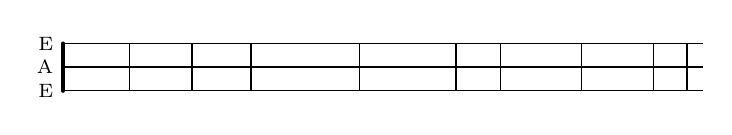
\begin{tikzpicture}[
  ynode/.style={draw=red!50,circle,fill=red!50,scale=.35,inner sep=1pt,minimum size=1.7em},
  zbar/.style={shorten >=-3,shorten <=-3,line width=6,round cap-round cap},
  znode/.style={white,draw=black,circle,fill=black,scale=.4,inner
    sep=1pt,minimum size=1.7em}
  ]

  %%%% Draw the base and set coordinates %%%%
  \begin{scope}[xscale=-15,yscale=.3,line width=.5]

    \xdef\x{1}
    
    %% Left line (nut):
    \draw[line width=1.5,cap=round] (1,1) -- (1,3);
    
    \foreach \fret in {1,2,...,13}{
      %% Set coordinate for each string
      \foreach \str in {1,2,3}{
        \coordinate (\str-\fret) at (0.97193715634*\x,\str);
      }
      
      %% Set coordinate for the text above
      \coordinate (Top-\fret) at (0.97193715634*\x,7);
      
      %% Compute the position of the fret
      \pgfmathsetmacro\x{\x * 0.94387431268}
      \xdef\x{\x}
      
      %% Draw the fret, if it is one of the frets on the phin:
      \foreach \test in {1,2,3,5,7,8,10,12,13}{
        \ifthenelse{\equal{\fret}{\test}}{
          \draw (\x,1) -- (\x,3);
        }{}
      }
      
    }

    %% Draw each string:
    \foreach \str in {1,2,3}{
      \draw (1,\str) -- (0.97153194115*\x,\str);
      \coordinate (start\str) at (1,\str);
    }

    %% Note names for open strings:
    \foreach \str/\note in {1/E,2/A,3/E}{
      \node[anchor=east] at (start\str) {\scriptsize\note};
    }

  \end{scope}

  %% \node[znode] at (2-3) {\textbf{C}};
  %% \node[znode] at (3-3) {\textbf{G}};

  %% Draw the mark on the guitare
  %% \foreach \f in {3,5,7,9,15,17}{
  %%   \draw[black!20,fill=black!10] ($(3-\f)!.5!(4-\f)$) circle (.08);
  %% }
  %% \draw[opacity=.20,fill,fill opacity=.10] (2-12) circle (.08) (5-12) circle (.08);

\end{tikzpicture}
\end{document}
